\documentclass[12pt]{article}

\usepackage{setspace}
\usepackage{caption}
\usepackage{subcaption}
\usepackage{float}
\usepackage{makecell}
\usepackage{amsmath}
\usepackage{graphicx}
\usepackage{subfig}
\graphicspath{ {./images/} }
\usepackage[utf8]{inputenc}
\usepackage[russian]{babel}
\usepackage{geometry}
 \geometry{
 a4paper,
 left=20mm,
 right=20mm,
 top=20mm,
 bot=20mm,
 }

\begin{document}

\begin{titlepage}
\begin{center}
    НАЦИОНАЛЬНЫЙ ИССЛЕДОВАТЕЛЬСКИЙ УНИВЕРСИТЕТ ИТМО \\
    Факультет систем управления и робототехники \\
    \vspace*{10\baselineskip}
    {\LARGEЭлектротехника} \\
    \ \\
    \ \\
    \begin{spacing}{1.5}
    {\large Лабораторная работа №21 \\
    СИНТЕЗ ПРЕОБРАЗОВАТЕЛЯ ДВОИЧНОГО (ДВОИЧНО-ДЕСЯТИЧНОГО) КОДА В СЕМИСЕГМЕНТНЫЙ \\
    \ \\
    Вариант 3R382}
    \end{spacing} \\
    \ \\
    \vspace*{10\baselineskip}
    \hfill {Студент: Кирбаба Д.Д.\ \ \ \ \ \ \ \ \ } \\
    \hfill {Группа: R3338\ \ \ \ \ \ \ \ \ \ \ \ \ \ \ \ \ \ \ \ \ } \\
    \hfill {Преподаватель: Китаев Ю.В.} \\
    \mbox{}
    \vfill {г. Санкт-Петербург\\2023}
\end{center}
\end{titlepage}

\subsection*{Цель работы}
Изучение преобразователей кодов.

\subsection*{Ход работы}

\begin{figure}[H]
    \centering
    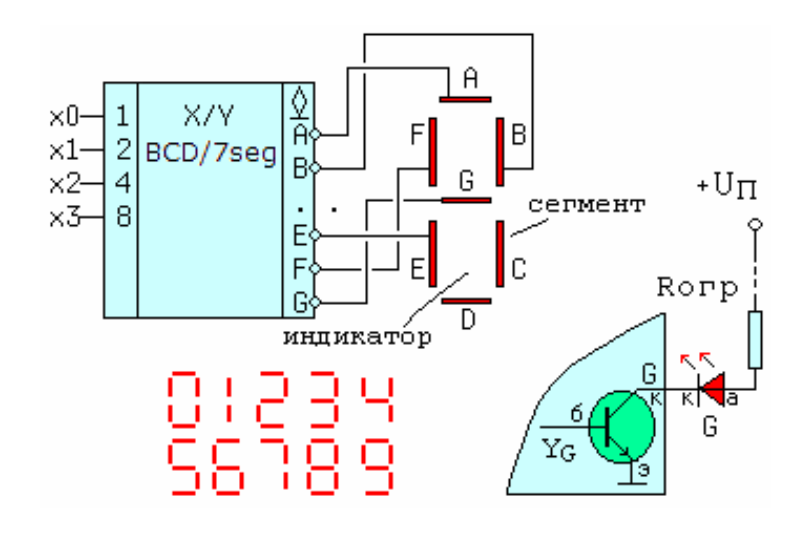
\includegraphics[width=0.5\textwidth]{main_scheme.png}
    \caption{Блок-схема преобразователя и фрагмент подключения отдельного светодиода (сегмента).}
    \label{fig:main_scheme}
\end{figure}

Заполним таблицу истинности преобразователя:
\begin{figure}[H]
    \centering
    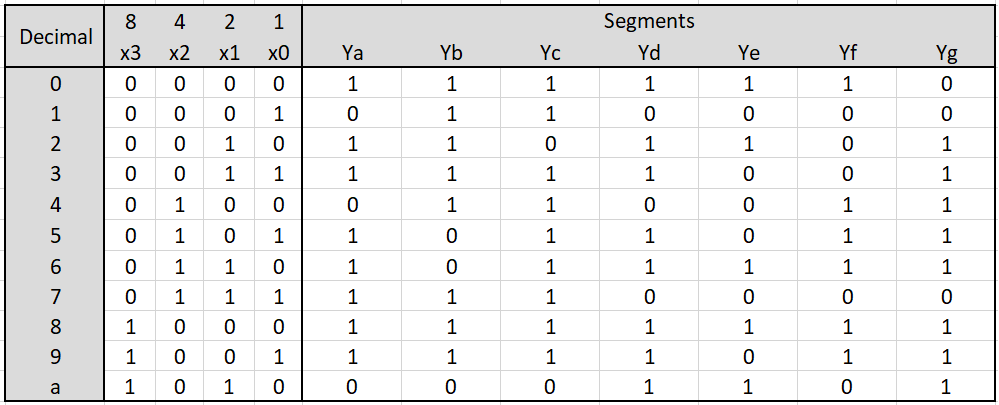
\includegraphics[width=0.8\textwidth]{true_table.png}
    \caption{Таблица истинности преобразователя.}
    \label{fig:true_table}
\end{figure}

В соответствии с вариантом $3R382$ необходимо выполнить работу для 3-х сегментов ЖК дисплея $A, \ B, \ E$. \\
Набор высвечиваемых цифр: $0123456789a$. \\
\ \\

Составим таблицу Карно и уравнения для каждого из трех заданных сегментов:
\begin{figure}[H]
    \centering
    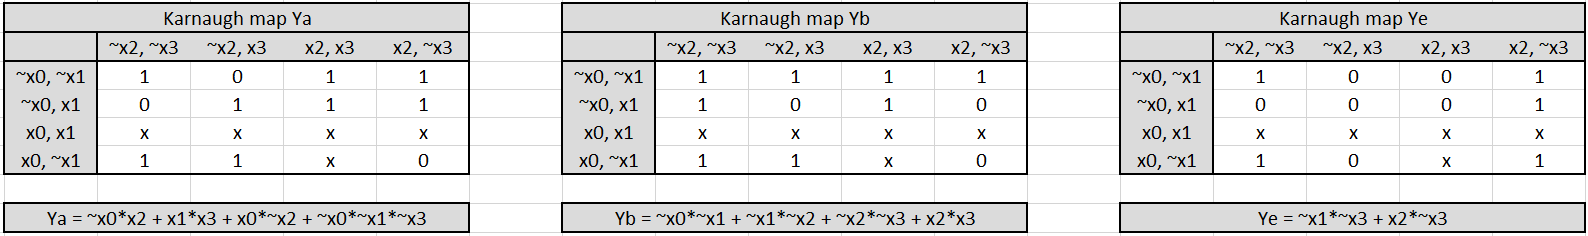
\includegraphics[width=\textwidth]{kar_maps.png}
    \caption{Таблицы Карно и уравнения для 3-х сегментов.}
    \label{fig:kar_maps}
\end{figure}

\begin{figure}[H]
    \centering
    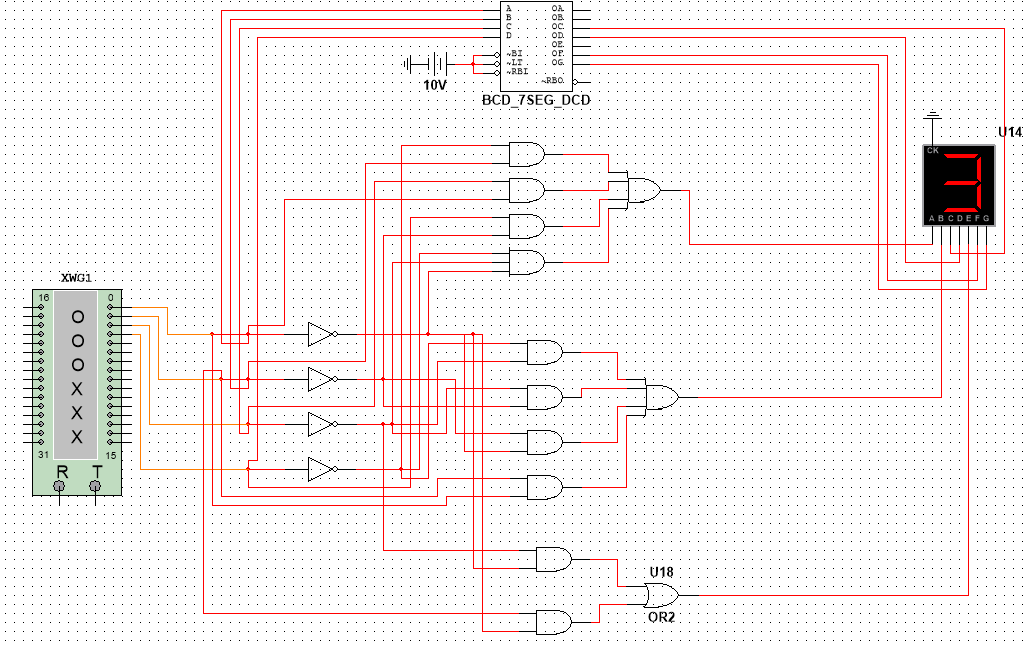
\includegraphics[width=\textwidth]{scheme_sim.png}
    \caption{Построенная блок-схема моделирования.}
    \label{fig:scheme_sim}
\end{figure}

Моделируя данную схему, свечение сегмента в соответствующих кодах преобразователя соответствует желаемому.

\subsection*{Выводы}
В данной работе был проведен синтез преобразователя двоичного кода в семисегментный. \\
В начале работы была построена требуемая таблица истинности для корректного вывода результата на сегменты. Затем, по ней были построены карты Карно и соответствующие уравнения для функций $Ya, \ Yb, \ Ye$. \\
Сконструированные уравнения были построены в модели и по результатам моделирования я убедился, что задание выполнено верно, так как все десятичные цифры на экране корректно отображаются по задаваемым двоичным кодам.

\end{document}